\documentclass{article}
\usepackage{tikz}

\newcommand{\scaffolding}{\draw [->] (0,-0.5) --(14,-0.5);
\draw[thick] (7,-0.5)--(10,-0.5);

\foreach \x in {1,4,7,10,13}
\draw(\x cm,3pt - 0.5cm) -- (\x cm, -3pt - 0.5cm);
}

\begin{document}

\subsection*{CEO succession}
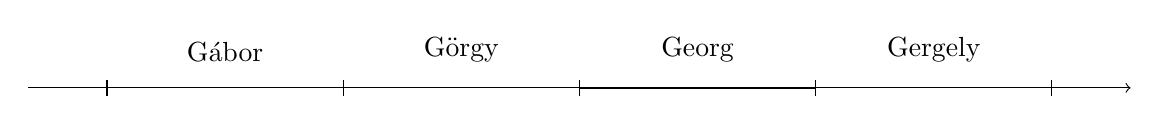
\begin{tikzpicture}
\scaffolding
\draw (2.5,-0.5) node[above=6pt, align=center] {Gábor};
\draw (5.5,-0.5) node[above=6pt, align=center] {Görgy};
\draw (8.5,-0.5) node[above=6pt, align=center] {Georg};
\draw (11.5,-0.5) node[above=6pt, align=center] {Gergely};
\end{tikzpicture}

\subsection*{Specific knowledge}
\begin{tikzpicture}
\scaffolding
\draw [red](0,0)--(7,0)--(7,3)--(10,3)--(10,0)--(14,0);
\end{tikzpicture}

\subsection*{Technology transfer}
\begin{tikzpicture}
\scaffolding
\draw [red](0,0)--(7,0)--(7,3)--(14,3);
\end{tikzpicture}

\subsection*{Reorganization}
\begin{tikzpicture}
\scaffolding
\draw [red](0,0)--(4,0)--(4,1)--(7,1)--(7,2)--(10,2)--(10,3)--(14,3);
\end{tikzpicture}

\end{document}